\section{Polymer Physics}

A polymer is a biomolecule made up of building blocks called monomers, linked together to
from a chain. In our simple mathematical model the configuration of this chain is
determined by the position vector of each monomer, denoted as $\{\boldsymbol{r}_0,
    \boldsymbol{r}_1, \dots,
\boldsymbol{r}_N\}$.  The link between each consecutive pair of monomers is called the
bond-vector, defined as
$\boldsymbol{u}_i = \boldsymbol{r}_i - \boldsymbol{r}_{i-1}$. During this discussion we
will assume these bonds to be inextensible, i.e. having a fixed
bond length of $|\boldsymbol{u}_i| = a$.

Various different models can be used to describe a polymer. The simplest version is
called the Freely Jointed Chain (FJC). This model is an example of an ideal flexible
polymer, in which excluded volume interactions or polymer bending rigidity are not taken
into account.  In this model, it is assumed that each bond-vector is completely
uncorrelated with its adjacent bonds. Mathematically this is represented by assigning the
bond-vector orientation a uniform probability distribution
\begin{equation}
    g(\boldsymbol{u}) = \frac{1}{4 \pi a}
    \delta(|\boldsymbol{u}| - a), \\
\end{equation}
where $a$ is the fixed bond length.

\begin{figure}[h!]
    \centering
    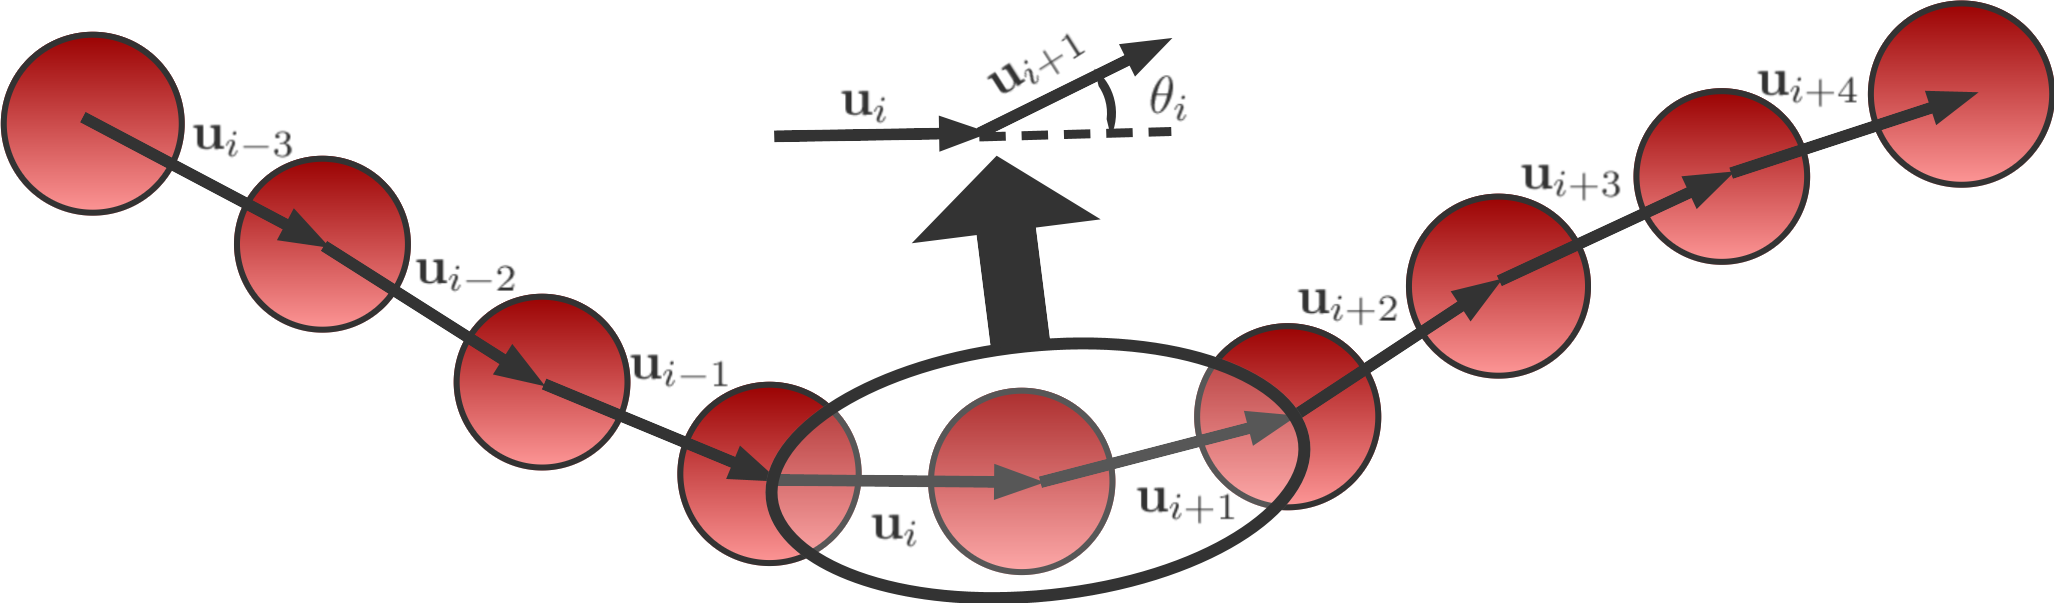
\includegraphics[width=0.95\linewidth]{Figures/kratky.png}
    \vspace{0.3cm}
    \caption[Illustration of the Kratky-Porod model.]{Kratky-Porod model. The angle
    between consecutive bonds, as highlighted in the
    figure, is used to impose bending rigidity in the polymer.}
    \label{fig:kratky}
\end{figure}

The above described model provides a relatively accurate description of long polymers.
However, the assumption that consecutive monomers are uncorrelated becomes
problematic at small length scales. The Kratky-Porod model \cite{Kratky1949}, or discrete
wormlike chain,
solves this problem by taking the energetic cost of bending the polymer into
account. Mathematically this is done by introducing a bending rigidity between
neighbouring bonds in the form of a coupling constant, $\kappa >0$. Each polymer
configuration is assigned an energy using the equation,
\begin{equation}
    E_{WLC}= -\kappa \sum_{i=1}^{N} \boldsymbol{\hat{u}_i} \cdot
    \boldsymbol{\hat{u}}_{i+1}
    = -\kappa
    \sum_{i=1}^{N} \cos\theta_i,
    \label{wlc}
\end{equation}
where $\boldsymbol{\hat{u}} = \boldsymbol{u}/a$ is the unit bond-vector and $\theta_i$ is
the angle between neighbouring bond-vectors $\boldsymbol{\hat{u}_i}$ and
$\boldsymbol{\hat{u}_{i+1}}$, see Figure \ref{fig:kratky}. The lowest energy state of
this discrete wormlike chain is
a straight rodlike configuration, where the bond angles $\theta_i$ are minimized.

To calculate the bond-vector correlation function,  we first determine the partition
function, $Z_{WLC}$, of the system. Identifying the single monomer contributions, this
quantity factorises into a product of single bond-vector partition functions as
\begin{equation}
    \begin{aligned}
        \label{210}
        Z_{\mathrm{WLC}}(N, T)
        &= \int_{0}^{\pi}\dots \int_{0}^{\pi} d \theta_1 \dots d \theta_N \sin \theta_1 \dots
        \sin \theta_N\ e^{\beta \kappa \sum_{i=1}^{N-1} \cos\theta_i}\\
        &= \left[\int_{0}^{\pi} d \theta \sin \theta e^{\beta \kappa \cos
        \theta}\right]^{N}\\
        &= \left[Z_{\mathrm{WLC}}(1, T)\right]^{N},
    \end{aligned}
\end{equation}
where $\beta=1/\kappa_b T$ is the inverse temperature. It rests us to determine the
single bond-vector partition function. Carrying out the integration yields the result,
\begin{equation}
    Z_{\mathrm{WLC}}(1, T)=\int_{0}^{\pi} d \theta e^{\beta \kappa \theta}=\frac{2
    \sinh(\beta \kappa)}{\beta \kappa}.
\end{equation}
%\begin{equation}
%    \left\langle\cos \theta_{i+1}\right\rangle
%    =\frac{\partial \log Z_{\mathrm{WLC}}(1, T)}{\beta \partial \kappa}.
%\end{equation}
From the found partition function we can now determine the bond-vector correlation
function. Using the definition of the partition function, we determine the average cosine
of the angle between consecutive bonds to be,
\begin{equation}
    \begin{aligned}
    \left\langle\cos \theta_{i+1}\right\rangle
    &=\frac{\partial \log Z_{\mathrm{WLC}}(1, T)}{\partial(\beta \kappa)}\\
    &= \frac{1}{\tanh(\beta \kappa)} - \frac{1}{\beta \kappa}.
    \end{aligned}
\end{equation}
Studying the conformation of polymers is often times done assuming a low
temperature or large bending rigidity, where we find
that the above expression simplifies. In the limit, $\beta \kappa \gg 1$, the lowest
order approximation yields,
\begin{equation}
    \langle\cos \theta\rangle \approx 1-\frac{1}{\beta \kappa}.
\end{equation}
Decomposing the bond-vector $\boldsymbol{\hat{u}}_{n+1}$ in terms of an orthonormal
basis, defined by the normal and tangential directions of the preceding vector
$\boldsymbol{\hat{u}}_{n+1}$, gives
\begin{equation}
\boldsymbol{\hat{u}}_{n+1} = \boldsymbol{\hat{u}}_{n} \cos \theta_{n} +
\boldsymbol{\hat{u}}_{n}^{\perp} \sin \theta_{n}.
\end{equation}
This decomposition allows us to express the correlation between distant bond-vectors in
terms of the correlation between neighbouring bond-vectors. The factorisation
yields
\begin{equation}
\begin{aligned}
    \left\langle\boldsymbol{\hat{u}}_{i} \cdot \boldsymbol{\hat{u}}_{i+m}\right\rangle
    &=\left\langle\boldsymbol{\hat{u}}_{i} \cdot
        \boldsymbol{\hat{u}}_{i+m-1}\right\rangle\left\langle\cos
    \theta\right\rangle = \dots =\langle\cos \theta\rangle^{m},
    % &=\exp \bigg{[} -\frac{n a}{l_{b}} \bigg{]},
\end{aligned}
\end{equation}
where we used the fact that the sinusoidal terms vanish due to symmetry.
Exploring this result in the limit, $\beta \kappa \gg 1$, we find the expression
\begin{equation}
    \left\langle\boldsymbol{\hat{u}}_{i} \cdot \boldsymbol{\hat{u}}_{i+m}\right\rangle =
    e^{m \log(1 - \frac{1}{\beta \kappa})} \approx e^{-na/l_p},
\end{equation}
introducing a new polymer quantity, the bending persistence length
\begin{equation}
    l_b \equiv \frac{a \kappa}{k_{b} T}.
    \label{eq:persistance}
\end{equation}
This general result in polymer physics states that the correlations between bond-vectors
exponentially decays. The defined quantity represents the characteristic
length scale over which the correlations between bond-vectors are lost.

Two limiting cases can be explored. Firstly, in the
case where the persistence length is much larger then the polymer's length, $l_p \gg na$,
all bond-vectors are correlated, i.e. the polymer approximates a straight rod. For the
reverse case, where $l_p \ll na$, it can easily be shown that the polymer behaves as a
stochastic walk.

The persistence length is a central result in the theory of polymer physics, providing a
measurable quantity related to the bending rigidity of a polymer. During the
simulations performed in this thesis, the notion of bending persistence length is used to
discuss the flexibility of the DNA polymer.

%The end-to-end vector $\boldsymbol{R}$ in the continuum limit. For example can be
%rewritten using the arc-length parameter $s$ where $0 \leq s \leq L$ and $L = Na$ as:
%\begin{equation}
%    \label{hoi}
%    \langle\widehat{u}(q) \cdot \widehat{u}(q+s)\rangle= e^{-s / l_{\mathrm{p}}}.
%\end{equation}
%The continuum version of the end-to-end vector
%\begin{equation}
%    \boldsymbol{R}=\int_{0}^{L} \widehat{u}(s) d s.
%\end{equation}

%\begin{equation}
%\begin{aligned}
%    \left\langle\boldsymbol{R}^{2}\right\rangle
%    &= \int_{0}^{L} d s d s^{\prime}\left\langle\widehat{u}(s) \cdot
%  \widehat{t}\left(s^{\prime}\right)\right\rangle \\
%    &= 2 l_{\mathrm{b}} L\left\{1-\frac{l_{\mathrm{b}}}{L}\left(1-e^{-L /
%l_{\mathrm{b}}}\right)\right\}.
%\end{aligned}
%\end{equation}
